\chapter{Validation, Traction, and the Scalable Startup}

This lecture is interview-format rather than blackboard-format, but it still unfolds with a clear quantitative discipline. We are first shown the entrepreneurial stakes in broad outline: ownership, rejection, wealth, and the prospect of building something saleable. Then the lecture narrows to John Abraham and becomes more exact. Before we build, we validate. Before we raise, we show traction. Before we scale, we decide where founder time is actually most valuable. The mathematics here is therefore modest and deliberate: a few timelines, a few inequalities, and several logical chains that compress the lecture's operating rules without pretending that the speaker gave a formal theorem.

\section{Opening Montage and the Entrepreneurial Stakes}

\paragraph{Anecdote.} The lecture opens in motion. We are on the way to meet John Abraham, and the host frames the encounter through a cluster of practical questions: how a founder starts, grows, sells, raises capital, and carries lessons from a first company into a second one.

\paragraph{Claim.} The early montage does two things at once. It promises that this will be about more than inspiration, and it quietly introduces a principle that will remain in the background all the way through: large wealth usually comes with ownership. In the teaser material, the move from seven figures to eight is not explained as a matter of working a little harder at the same wage. It is explained as a matter of getting equity in a company or building a company of our own.

We may compress that opening claim into the heuristic relation
\begin{equation}
\text{path from seven to eight figures}
\;\approx\;
\text{equity in somebody else's company}
\;\;\text{or}\;\;
\text{equity in one's own company}.
\end{equation}

\paragraph{Mechanism.} At this stage the lecture is still setting the stakes rather than proving anything. We are being told what kinds of questions matter: where ownership enters, how capital appears, how scale becomes possible, and what makes a business worth buying.

\section{Public Advice, Rejection, and the Return to Abraham}

\paragraph{Anecdote.} Before the sustained founder interview begins, the lecture samples several nearby voices. A retired tech salesman describes a year in which stock options pushed earnings into eight figures. A government consultant says that success requires assertiveness joined to professionalism, and that relationships should be treated as relationships rather than as networking. Another operator, in a niche industrial business, says that one must find a niche, work hard, and cut losing directions early.

There is also a rejection sequence. The hosts speak to strangers, get turned away, and then pause to make the principle explicit: rejection is part of the process; every no moves us closer to a yes.

\paragraph{Claim.} These fragments are not the chapter's main argument, but they matter for rhythm. They create a field of entrepreneurial folklore and lived experience before the lecture narrows to a more coherent founder method. They also introduce motifs that Abraham's interview will later absorb and reorganize: ownership, rejection, niche focus, and long-term relationships.

\paragraph{Mechanism.} We are not yet inside a systematic model. We are being shown the raw environment in which founders operate. That environment is noisy, social, and uncertain. The lecture then pivots back to Abraham precisely because his story can turn that noisy environment into a sequence of practical tests.

\section{Meeting John Abraham and the First Step from Idea to Action}

\paragraph{Anecdote.} The hosts explain how they first encountered Abraham in Austin, overheard him talking business, and later returned to record him properly. Abraham then gives the compressed version of his own business trajectory:
\begin{equation}
t_{\text{launch}} = 2014,
\qquad
t_{\text{exit}} = 2018,
\qquad
\Delta t = t_{\text{exit}} - t_{\text{launch}} = 4 \text{ years}.
\end{equation}
He had entered tech through sales, launched an application, exited in 2018, and is now building Haymaker.

\paragraph{Claim.} This timeline is short, but it establishes the right kind of authority. The lecture is no longer speaking in the general language of hustle or ambition. It is speaking through somebody who has already built, sold, and started again.

\begin{definition}
We use \(\mathrm{TAM}\) for the total addressable market. In this lecture \(\mathrm{TAM}\) is not computed numerically; it functions as a discipline. Before we build, we ask whether the problem belongs to a market broad enough to sustain a company.
\end{definition}

\begin{definition}
We use \(\mathrm{MVP}\) for the early product built after some market evidence appears. Abraham says ``minimally viable product.'' We keep the abbreviation \(\mathrm{MVP}\) and preserve his sequence: evidence first, build second.
\end{definition}

\paragraph{Anecdote.} The host now asks the first truly operational question: how do we move from a good idea to actual execution?

\subsection{Question \& Answer}

\paragraph{Question.} What is the first step from idea to action?

\paragraph{Answer.} The answer is deliberately anti-romantic. Before creating anything, we need to understand the viability of the product and the \(\mathrm{TAM}\). Then we should interview as many potential clients as possible, especially the decision-makers in the relevant space.

\paragraph{Mechanism.} The lecture gives us a clear sequence:
\begin{align}
\text{Need observed}
&\Rightarrow \text{interview decision-makers},\\
\text{Interview evidence}
&\Rightarrow \text{clearer statement of pain},\\
\text{Pain with business value}
&\Rightarrow \text{pilot commitment},\\
\text{Pilot commitment}
&\Rightarrow \text{build the }\mathrm{MVP}.
\end{align}
And it is important that the sequence not be inverted. We do not begin by pressing for a sale. We begin by asking what the client's challenges are and what solving them would mean for the company. Only after that discussion has clarified the value do we ask for something stronger, namely a willingness to pilot the solution.

\begin{figure}
\centering
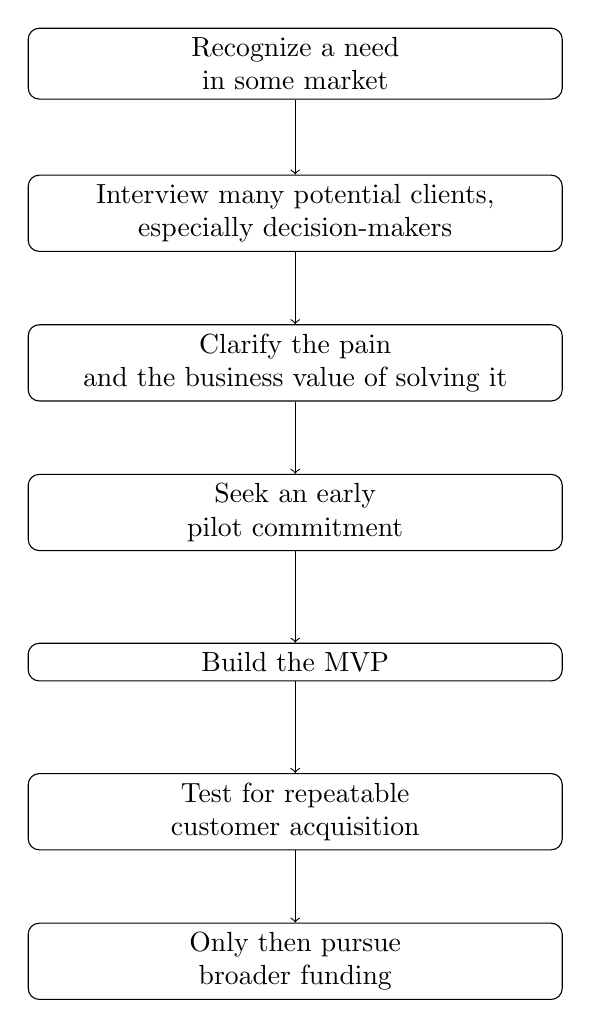
\begin{tikzpicture}
\node[draw, rounded corners, align=center, text width=0.54\linewidth] (n1) at (0,0) {Recognize a need\\in some market};
\node[draw, rounded corners, align=center, text width=0.54\linewidth] (n2) at (0,-1.9) {Interview many potential clients,\\especially decision-makers};
\node[draw, rounded corners, align=center, text width=0.54\linewidth] (n3) at (0,-3.8) {Clarify the pain\\and the business value of solving it};
\node[draw, rounded corners, align=center, text width=0.54\linewidth] (n4) at (0,-5.7) {Seek an early\\pilot commitment};
\node[draw, rounded corners, align=center, text width=0.54\linewidth] (n5) at (0,-7.6) {Build the \(\mathrm{MVP}\)};
\node[draw, rounded corners, align=center, text width=0.54\linewidth] (n6) at (0,-9.5) {Test for repeatable\\customer acquisition};
\node[draw, rounded corners, align=center, text width=0.54\linewidth] (n7) at (0,-11.4) {Only then pursue\\broader funding};

\draw[->] (n1) -- (n2);
\draw[->] (n2) -- (n3);
\draw[->] (n3) -- (n4);
\draw[->] (n4) -- (n5);
\draw[->] (n5) -- (n6);
\draw[->] (n6) -- (n7);
\end{tikzpicture}
\end{figure}

\begin{remark}
This diagram is an editorial reconstruction of the spoken sequence, not a claim about on-screen board content.
\end{remark}

\section{When Does an Idea Become a Business?}

\paragraph{Anecdote.} The next move is exactly right. Once we have an idea, a team, and some money being spent, we naturally want to know whether we should continue. This is the lecture's first real tension. The founder may feel that the problem is important, but the business test has not yet been met.

\subsection{Question \& Answer}

\paragraph{Question.} At what point do we know that the idea is good enough to keep investing in?

\paragraph{Answer.} Abraham's answer is strict. A substantial problem is not enough. Until we know how to get customers at scale, we do not yet have a great business idea.

We may write the negative and positive forms side by side:
\begin{equation}
\text{Substantial problem alone}
\;\not\Rightarrow\;
\text{great business},
\end{equation}
whereas
\begin{equation}
\text{Great business idea}
\;\Rightarrow\;
\bigl(\text{substantial problem}\bigr)
\land
\bigl(\text{customer acquisition can scale}\bigr).
\end{equation}

\paragraph{Mechanism.} This is where the lecture draws its sharpest distinction. A painful problem may exist and still fail to become a company. The decisive difference is not private conviction but the existence of a repeatable path from product to customer. In that sense, the question ``Is this a good idea?'' is too soft. The harder and more useful question is ``Can we build a repeatable customer-acquisition machine around this problem?''

\paragraph{Mechanism.} We may summarize the test as a short derivation:
\begin{enumerate}
\item Identify a real problem.
\item Verify that decision-makers recognize it as costly or urgent.
\item Seek proof that the solution would be tried in practice.
\item Look for a repeatable path to customers.
\item Only then promote the idea from interesting problem to investable business.
\end{enumerate}

\section{Perfectionism, Failure, and the Capital Test}

\paragraph{Anecdote.} Having tied judgment to the market, the lecture immediately turns to the founder habits that prevent real market contact. The host asks about perfectionism and analysis paralysis, and later about repeated failure and adversity.

\paragraph{Claim.} Abraham treats perfectionism not as refinement but as insecurity. We do not want anyone calling the baby ugly, so we never show anyone the baby. That is a psychologically vivid way of saying that hidden products do not generate information.

We may express the contrast schematically as
\begin{align}
\text{imperfect release}
&\Rightarrow \text{feedback}
\Rightarrow \text{course correction},\\
\text{hidden product}
&\Rightarrow \text{no feedback}
\Rightarrow \text{no correction}.
\end{align}

\paragraph{Mechanism.} This prepares the ground for the lecture's treatment of failure. Rejection and adversity are not external interruptions to the entrepreneurial process; they are among the mechanisms by which the founder learns. The earlier street-rejection segment now acquires a second function. It is not merely atmosphere; it is a miniature of what product learning will look like later.

\paragraph{Claim.} The lecture then widens the frame. Entrepreneurship is a journey before it is a destination. The public may celebrate the money attached to an exit or an IPO, but the speaker insists that the more durable gain is the operator we become through repeated confrontation with obstacles.

\paragraph{Anecdote.} From there the lecture pivots back to one of the opening teaser questions: raising capital.

\subsection{Question \& Answer}

\paragraph{Question.} What do investors really need to see before funding a business?

\paragraph{Answer.} There is no magic threshold. The lecture refuses any sacred number. Instead, investment readiness is a conjunction of signals:
\begin{equation}
\text{Ready for investment}
\;\Rightarrow\;
\bigl(\text{potential}\bigr)
\land
\bigl(\text{repeatable customer acquisition}\bigr)
\land
\bigl(\text{plan}\bigr).
\end{equation}

\paragraph{Mechanism.} The order matters. We build and test as cheaply as possible. If some revenue appears, we reinvest into broader traction. Only after we have evidence do we take the business out for investment. The lecture's metric-language is still cautious, but it is unmistakably directional. Ideally both revenue and recurring revenue move upward month by month:
\begin{align}
R_{t+1} &> R_t,\\
\mathrm{MRR}_{t+1} &> \mathrm{MRR}_t.
\end{align}
Here \(R_t\) denotes period revenue and \(\mathrm{MRR}_t\) denotes monthly recurring revenue at period \(t\).

\begin{remark}
These inequalities are careful editorial encodings of Abraham's verbal criterion that revenue and \(\mathrm{MRR}\) should be moving up month by month. They are not quoted formulas from a board.
\end{remark}

\section{Scaling, Channels, Saleability, and Haymaker}

\paragraph{Anecdote.} After the capital question, the lecture advances to the next one in sequence: how do we scale?

\paragraph{Claim.} Abraham's answer is not mystical. It is a time-allocation rule. If a task can be outsourced for less than the founder's effective hourly value, then the task should be outsourced.

Let \(r_F\) be the founder's effective hourly rate and \(c_{\text{task}}\) the outside cost rate of the task. Then the lecture's rule is
\begin{equation}
c_{\text{task}} < r_F
\;\Rightarrow\;
\text{outsource the task}.
\end{equation}

\paragraph{Mechanism.} This inequality does not solve accounting for us, but it does identify the controlling variable. Scale begins when the founder stops spending premium time on low-leverage work. If the work instead requires a permanent employee, the lecture adds a second piece of discipline: put the role in the forecast, budget for it, and grow the team deliberately rather than accidentally.

\paragraph{Anecdote.} The host then asks about marketing, and the lecture makes an important branch distinction.

\paragraph{Claim.} Marketing depends on the type of customer. In the lecture the split is practical:
\begin{align}
\text{Enterprise play}
&\Rightarrow
\text{email + direct outreach + possibly cold calling},\\
\text{Consumer play}
&\Rightarrow
\text{social media as a central channel}.
\end{align}

\paragraph{Mechanism.} This is fully consistent with the earlier validation logic. We interview decision-makers first because the go-to-market path depends on the buyer we are trying to reach. Channel choice is therefore downstream from customer structure, not an ornamental add-on at the end.

\paragraph{Anecdote.} The lecture then turns to the problem of making a company saleable. Abraham had already exited once, so the host asks what that process looks like and how we should prepare for it.

\paragraph{Claim.} The answer is again operational rather than theatrical. The best way to set up a company to be sold is to keep building revenue and moving the bottom line efficiently. If that machine is working, investors and acquirers will notice.

We may compress the claim as
\begin{equation}
\text{efficient revenue growth}
\;\Rightarrow\;
\text{investment or acquisition attention}.
\end{equation}

\paragraph{Mechanism.} The lecture also insists that no founder has a universal advisor. Motivation may come from one person, but domain knowledge has to come from domain experts: sales mentors for sales, specialists for other functions, and a circle of advisors rather than a single omniscient guide.

\paragraph{Anecdote.} Finally, the chapter returns to Haymaker itself. Abraham describes it as a marketplace, similar in form to Airbnb, but focused on temporary office and meeting spaces. The company started closer to coworking and then pivoted during the pandemic toward meeting spaces as distributed work reduced the appetite for permanent footprints.

\paragraph{Mechanism.} That ending is pedagogically well chosen. We do not finish with a slogan; we finish with a live example of the earlier method. A market shifts, a need becomes visible, the company repositions, and the founder follows the evidence.

\section{Summary}

The lecture proceeds in a strict order, even though it is delivered in an interview voice. It begins by placing entrepreneurship in a field of practical questions about ownership, rejection, and success. It then narrows to Abraham's case and turns that field into a sequence. First we validate demand through interviews with decision-makers. Then we distinguish a meaningful problem from a scalable business by asking whether customer acquisition can repeat. Then we refuse perfectionism in favor of feedback, and we treat failure as part of the learning apparatus rather than as a verdict. After that, capital is allowed to enter, but only after evidence of potential, repeatable acquisition, a plan, and upward-moving revenue or \(\mathrm{MRR}\). Finally, scale appears as leverage, channel selection, clean operating performance, and the deliberate use of advisors.

That sequence is the chapter's durable contribution. The lecture is not a bundle of startup slogans. It is a compact operating philosophy: validate before we build, prove traction before we fund, and protect leverage as we scale.